\section{Framework: Trajectories, Metrics, and the Signature Matrix}
\label{sec:framework}

\subsection{Trajectories}

Given an LLM $f$ with $L$ transformer layers and hidden dimension $d$, a prompt $p$,
and a decoding strategy (greedy unless stated otherwise), we run $f$'s standard
generation loop and record, at every generated token $t \in \{1,\dots,T\}$, the
residual-stream hidden state at every layer
$\ell \in \{0, 1, \dots, L\}$ (index $0$ is the embedding output, $\ell{=}L$ is the
final transformer block). We collect last-position vectors only, giving a tensor
\begin{equation}
\label{eq:trajectory-tensor}
  H \in \mathbb{R}^{T \times (L+1) \times d}.
\end{equation}
A trajectory is one such tensor. The per-layer projection
$H_{:,\ell,:} \in \mathbb{R}^{T\times d}$ is the $\ell$-th \emph{per-layer
trajectory}.

\paragraph{Intuition.} At one fixed layer, this sequence is like tracing a pen
path through a high-dimensional space: each generated token is one point, a
step vector is the short line between adjacent points, and a turning angle asks
whether the path keeps going in the same direction or bends. The metrics below
do not claim that a model literally reasons in Euclidean space; they are compact,
reproducible summaries of how its residual states move while it generates an
answer.  Table~\ref{tab:notation} fixes the notation used below.

\begin{table}[tbp]
\centering
\small
\caption{Notation at a glance. All quantities are fixed before the controlled
evaluations in Section~\ref{sec:crosssteer-no-leakage}.}
\label{tab:notation}
\begin{tabular}{@{}lp{0.67\columnwidth}@{}}
\toprule
Symbol & Meaning \\
\midrule
$p_i, a_i$ & Prompt $i$ and its gold answer \\
$c_i$ & Exact-answer correctness indicator for one generated answer \\
$T, L, d$ & Generated-token count, transformer depth, and hidden width \\
$H^{(i)}$ & Generated-token hidden-state tensor for example $i$ \\
$\phi, S[\phi,\ell]$ & Trajectory function and its metric--layer correctness association \\
$v_\ell, \alpha$ & Layer-$\ell$ steering direction and its root-mean-square (RMS)-scaled strength \\
$I_c, I_v, I_l$ & Disjoint calibration, validation, and locked-test problem IDs \\
$N, K$ & Generic sample count in the algorithm; fixed experimental candidate-pool size \\
\bottomrule
\end{tabular}
\end{table}

\subsection{Geometric metrics}

We compute seven trajectory metrics, each producing a scalar per layer. All
computations use float32 even when $H$ is stored in bfloat16, since the inner
products and norms involved underflow in bfloat16 at $d \ge 1024$.

\paragraph{Length-derived.}
\begin{itemize}
\item $\textsc{TrajLen}(H_\ell) = \sum_{t=1}^{T-1} \lVert H_{t+1,\ell,\cdot} - H_{t,\ell,\cdot}\rVert_2$
\item $\textsc{StepNorm}(H_\ell) = \textsc{TrajLen}(H_\ell) / (T-1)$, the
mean step size. Unlike \textsc{TrajLen}, it does not add a term for every
extra generated token.
\end{itemize}

\paragraph{Curvature-derived.} Let
$v_t = H_{t+1,\ell,\cdot} - H_{t,\ell,\cdot}$ and
\begin{equation}
\label{eq:turning-angle}
\theta_t = \arccos\!\left(
  \frac{v_t \cdot v_{t+1}}{\lVert v_t\rVert_2 \lVert v_{t+1}\rVert_2}
\right)
\end{equation}
denote the discrete turning angle at interior step $t$.
Figure~\ref{fig:curvature-schematic} gives a two-dimensional sketch: a small
turning angle means adjacent displacement vectors point similarly, whereas a
large angle means the path changes direction sharply. The computation itself
uses the original layer-space vectors, not this projection.

\begin{figure*}[tbp]
\centering
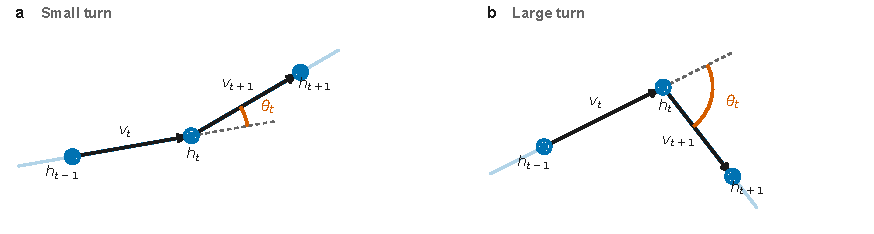
\includegraphics[width=0.78\linewidth]{figures/fig_curvature_schematic.pdf}
\caption{Curvature intuition.  The 2D sketch contrasts small and large turns;
$\theta_t$ is computed from adjacent displacements in the full layer space.}
\label{fig:curvature-schematic}
\end{figure*}

We report $\textsc{CurvMean}$ (the mean of $\theta_t$), $\textsc{CurvVar}$ (sample
variance), and three quantiles $\textsc{CurvMax}$, $\textsc{Curv}_{p90}$,
$\textsc{Curv}_{p99}$. These summarize the distribution of per-step angles
rather than accumulating travel over the whole path. Their sampling behavior can
still depend on how many steps a completion has, so the signature below applies
the same generated-length control to every displayed metric.

\subsection{Geometric signature}

Given a model $f$, a dataset $\mathcal{D}=\{(p_i, a_i)\}$ of prompts and gold
answers, and a correctness indicator $c_i \in \{0,1\}$ for the generated answer
to $p_i$, we define the \emph{geometric signature}
\begin{equation}
\label{eq:signature}
\begin{aligned}
  S(f, \mathcal{D}) &\in [0,1]^{|\Phi|\times (L+1)},\\
  S[\phi, \ell] &= \operatorname{AUC}\bigl(\{\phi(H^{(i)}_\ell)\}_i,\{1-c_i\}_i\bigr),\\
  &\hspace{7em}\phi\in\Phi.
\end{aligned}
\end{equation}
where $H^{(i)}_\ell$ is the per-layer trajectory of $f$ on $p_i$, $\Phi$ is the
fixed set of trajectory functions, and AUC measures how well higher metric
values rank \emph{incorrect} samples above correct ones. We use $1-c_i$ as the
positive label so that interpretation is uniform across functions:
$S[\phi,\ell] > 0.5$ means a high value of $\phi$ flags incorrect outputs;
$S[\phi,\ell]{<}0.5$ indicates the function is sign-flipped (a high value is
associated with correct outputs).

\paragraph{Length-residualized signature.}
Longer completions trivially inflate accumulated path length and can also change
the sampling distribution of per-step statistics. For every metric--layer cell,
we fit a linear nuisance model whose predictor is
$\log(1+\textsc{n-gen-tokens}_i)$, using the diagnostic data, and then compute
the AUC on the residuals. We call this the \emph{length-residualized AUC}; it is
not an AUC restricted to a particular false-positive-rate range. All signature
comparisons in Section~\ref{sec:phenomenon} use this same log-length
residualization. It removes the specified linear component in log length but
does not establish length invariance for nonlinear or extreme-value statistics.

\subsection{Signature distance}
For two signatures we define
\begin{equation}
\label{eq:signature-distance}
  d(S_1, S_2) = \lVert (S_1 - 0.5) - (S_2 - 0.5)\rVert_F,
\end{equation}
so that cells without signal in either model contribute zero. Both signatures must
be computed on the same dataset $\mathcal{D}$. Pairwise $d$ over a model family
yields the distance matrix used in Section~\ref{sec:phenomenon}.

\subsection{Signed orientation}
\label{sec:signed-orientation}

For a single trajectory-function row $\phi$, we also use the signature as a signed diagnostic:
\begin{equation}
\label{eq:signed-orientation}
\begin{split}
\ell^* &= \arg\max_\ell |S[\phi,\ell]-0.5|,\\
o_\phi(f) &= \operatorname{sign}\!\left(S[\phi,\ell^*]-0.5\right).
\end{split}
\end{equation}
Because AUC is computed with incorrect outputs as the positive class,
$o_\phi(f)>0$ means high values of $\phi$ are associated with incorrect generations, while
$o_\phi(f)<0$ means the function is sign-flipped and high values are associated with
correct generations. We record $o_{\textsc{CurvMean}}$ as a descriptive
calibration-time covariate for \textsc{CrossSteer}; it is not a compatibility
rule or a claimed mechanism.  The orientation is learned on labeled calibration
trajectories and then frozen; it is not computed from held-out answers.

\subsection{Inference-time procedures}
\label{sec:inference-procedures}

The diagnostic signature can be used in two logically distinct ways.  Both are
defined here before their controlled evaluations, so that an evaluation result
cannot retroactively change the method definition.

\subsubsection{\textsc{GeoVote}: trajectory-scored aggregation}
\label{sec:geovote-method}

Given a model $f$, a prompt $p$, and $N$ samples $\{x^{(i)}\}_{i=1}^{N}$ produced by
temperature sampling, we extract a per-trajectory scalar
$\mu^{(i)} = \phi(H^{(i)}_{\ell^*})$ for a calibrated trajectory function $\phi$,
layer $\ell^*$, and sign. If calibration says smaller values are more reliable, sample
$i$ receives $w^{(i)}=(\mu^{(i)}+\varepsilon)^{-1}$; otherwise it receives
$w^{(i)}=\max(\mu^{(i)},0)$. The answer string with the largest total weight
is returned:
\begin{equation}
\label{eq:geovote}
\hat{y}=\arg\max_{a}\sum_{i:x^{(i)}\to a}w^{(i)} .
\end{equation}
Aggregation groups candidates by parsed answer and returns the largest total
weight. That combinator is shared with the log-probability-weighted row in
Section~\ref{sec:geovote}; the weight map is not. Frozen \textsc{GeoVote} uses
the sign-dependent weights above, whereas the likelihood control uses
softmax-normalized log-probabilities.
Metric, layer, sign, and aggregation rule are selected on calibration questions
and frozen before held-out evaluation.

\begin{center}
\fbox{\begin{minipage}{0.94\columnwidth}
\small
\algtitle{\textsc{GeoVote}$(p,f,\phi,\ell^*,N)$}\label{alg:geovote}\par
\textbf{Input:} prompt $p$, model $f$, frozen metric $\phi$, layer $\ell^*$,
sign, and sample count $N$.\par
\textbf{1. Freeze.} Select the metric, layer, sign, and vote rule on calibration
questions.  Do not use held-out answers.\par
\textbf{2. Sample and score.} Draw $N$ solutions.  For each solution, extract
$H^{(i)}$, compute $\mu^{(i)}=\phi(H^{(i)}_{\ell^*})$, and convert the signed
score into a nonnegative weight $w^{(i)}$.\par
\textbf{3. Aggregate.} Group candidates by parsed answer and return the answer
with the largest total weight.  Reuse the identical candidate pool for every
comparison rule.\par
\textbf{Output:} one selected answer and the per-candidate audit record.
\end{minipage}}
\end{center}

\subsubsection{\textsc{CrossSteer}: source-direction intervention}
\label{sec:crosssteer-method}

Given a \emph{source} model $f_s$ with trajectories $\{H^{(i)}_{s}\}$ on a dataset
$\mathcal{D}$ with known correctness $\{c_i\}$, define the layer-$\ell$ steering vector
\begin{equation}
\label{eq:crosssteer}
\begin{aligned}
  v_\ell = \mathbb{E}_{i:\,c_i{=}1}\!\bigl[\overline{H^{(i)}_{s,\ell,:}}\bigr]
            - \mathbb{E}_{i:\,c_i{=}0}\!\bigl[\overline{H^{(i)}_{s,\ell,:}}\bigr]
            \in \mathbb{R}^d .
\end{aligned}
\end{equation}
where the inner expectation $\overline{\,\cdot\,}$ averages over the generated tokens
of trajectory $i$. For a target model $f_t$ that shares hidden dimension $d$ with
$f_s$, we run $f_t$'s inference with a forward hook at residual-stream layer $\ell$:
\begin{equation}
\label{eq:crosssteer-injection}
  h_\ell^{f_t}\ \mathrel{+}=\ \alpha\, v_\ell.
\end{equation}
Index $\ell$ runs from $0$ (embedding output) to $L$ (final block output);
injection at $\ell_0{\ge}1$ adds to the residual stream at block
$\ell_0{-}1$'s output, and $\ell_0{=}0$ would add at the embedding output.
Reported cells use $\ell_0\in\{14,20,24\}$.  In the controlled protocol,
the hook is applied only to generated decode steps (never prompt prefilling), and
the direction is RMS-normalized before applying $\alpha$.  Source correctness
labels are used only to build $v_\ell$ on calibration trajectories; held-out
target answers are not used by the hook.  A layer, strength, and schedule may be
chosen only on a disjoint validation split under the predeclared behavior guard,
and are then frozen for one locked evaluation.  This direct form assumes equal
hidden width. Cross-family transfer across different widths would need an
additional learned alignment, which we leave for future work.

\begin{center}
\fbox{\begin{minipage}{0.94\columnwidth}
\small
\algtitle{\textsc{CrossSteer}$(\mathcal{D}_s,f_s,f_t)$}\label{alg:crosssteer}\par
\textbf{Input:} labeled source-calibration trajectories, target-validation
questions, target model $f_t$, and a locked test split.\par
\textbf{1. Build directions.} At each layer, average the source trajectory over
generated tokens and subtract the incorrect mean from the correct mean to obtain
$\{v_\ell\}_{\ell=0}^{L}$.\par
\textbf{2. Freeze.} On disjoint target-validation questions, apply the
predeclared grid rule once to choose layer, RMS-scaled strength, and schedule.
Record the vector hash and freeze the choice.\par
\textbf{3. Intervene.} During target decoding only, add the selected
$\alpha v_\ell$ at the selected layer.  Never modify prompt-prefill states.\par
\textbf{4. Evaluate.} Compare the steered and unsteered outputs problem by
problem on the locked split.  Record accuracy, repairs, breaks, length,
repetition, stopping, and truncation.\par
\textbf{Output:} one locked paired comparison and its complete audit record.
\end{minipage}}
\end{center}

\subsection{Controlled evaluation protocol}
\label{sec:crosssteer-no-leakage}

Any reported steering gain must survive a strict separation between the ids
that supply correctness labels and the ids that supply evaluation labels.  We use
three disjoint splits: source-direction training ids $I_c$, validation ids $I_v$
for the fixed layer/strength/schedule selection rule, and a locked test $I_l$
that is generated exactly once after selection.  Every run records its source
ids, vector hash, model/tokenizer revision, prompt, and resolved decoding
configuration.  A source/evaluation overlap fails automatically and is treated
as exploratory.  On the locked test, comparisons are problem-paired and report
accuracy, repairs, breaks, a paired nonparametric bootstrap confidence interval,
exact paired test, and behavior diagnostics (length, repetition, answer-marker
position, stopping, and truncation).  Multiple formal comparisons receive the
predeclared family-wise correction.  A point estimate without these paired controls is not treated as confirmatory evidence.
